\documentclass[aspectratio=169]{beamer}

% because we need to claim weird things
\newtheorem{claim}{Claim}
\newtheorem{defn}{Definition}
%\newtheorem{lemma}{Lemma}
\newtheorem{thm}{Theorem}
\newtheorem{vita}{Vit\ae}
\newtheorem{qotd}{Quote of the Day}

\usepackage{algorithm}
\usepackage{algpseudocode}
\usepackage{listings}
\usepackage{color}
\usepackage{graphics}
\usepackage{ulem}
\bibliographystyle{unsrt}

% background image
\usebackgroundtemplate%
{%
    
\includegraphics[width=\paperwidth,height=\paperheight]{../artifacts/stemulus.pdf}%
}
\setbeamertemplate{caption}[numbered]
\lstset{%
	breaklines=true,
	captionpos=b,
	frame=single,
	keepspaces=true,
	showstringspaces=false
}

% page numbers
\addtobeamertemplate{navigation symbols}{}{%
    \usebeamerfont{footline}%
    \usebeamercolor[fg]{footline}%
    \hspace{1em}%
    \insertframenumber/\inserttotalframenumber
}

% presentation header
\usetheme{warsaw}
\title{Week 3: Unit Testing}
\author{Dylan Lane McDonald}
\institute{CNM STEMulus Center\\Web Development with PHP}
\date{\today}

\begin{document}
\lstset{language=Java}
\begin{frame}
\titlepage
\end{frame}

\begin{frame}
\frametitle{Outline}
\tableofcontents
\end{frame}

\section{Unit Testing}
\subsection{About Unit Testing}
\begin{frame}
\frametitle{Unit Testing}
Unit testing has already been alluded to in this set of slides. But a more complete definition would be:
\begin{defn}
A \textbf{unit test} is a function that tests another function (a \emph{unit}) for a specific set of inputs and conditions and expects a specific outcome and outputs.
\end{defn}

\pause
Notice the use of the word \textbf{unit} in the term unit test. In agile, programming units are the \textbf{smallest functionality possible} that accomplish the given task or objective. One keystone of agile design and methodologies is the fact that a problem is composed of many small units. This is what facilitates Agile's flexibility.
\end{frame}

\begin{frame}
\frametitle{Unit Testing Terminology}
Add all these terms to your lexicon.
\begin{itemize}
	\item \textbf{Assertion}: A testable condition the unit test is testing for. For example:
	\begin{itemize}
		\item \textit{Assert $x$ is in array $A$}
		\item \textit{Assert $x < y$}
		\item \textit{Assert $x$ is not \textbf{NULL}}
	\end{itemize}
	\item \textbf{Throws}: An assertion that succeeds if and only if an exception is thrown
	\item \textbf{Setup}: A function that sets up testing conditions to be run before the unit test is executed
	\item \textbf{Tear Down}: A function that destroys the test data created by setup or the unit test after the unit test is executed
\end{itemize}
\end{frame}

\subsection{Executing Unit Tests}
\begin{frame}
\frametitle{Unit Testing Process}
\begin{figure}
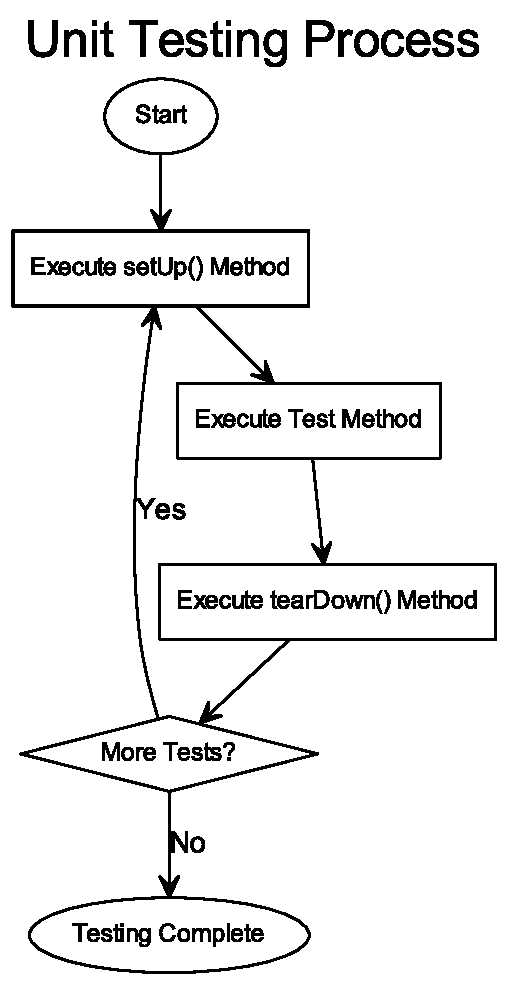
\includegraphics[scale=0.36]{../artifacts/unit-testing-flow.pdf}
\caption{Unit Testing Process}
\label{fig:flow}
\end{figure}
\end{frame}

%\subsection{Executing Unit Tests}
%\begin{frame}[fragile]
%\frametitle{QUnit Unit Test}
%\begin{lstlisting}[caption=QUnit Unit Test]
%test("hello test",
%   function() {
%      ok(1 == "1", "Passed!");
%   }
%);
%\end{lstlisting}
%QUnit unit tests take the form as seen in Listing 1. After setting up the HTML and JavaScript, units can be tested using the \texttt{test()} method. Full examples and document are at \url{http://qunitjs.com/}.
%\end{frame}
\end{document}